% Section: Mechanism (H3) — P8 commit 7.
% All numerical claims verified against:
%   - results/p7_t3_mechanism/t3_scalars.json
%   - results/p7_5_h3_loo/h3_loo_results.json
%   - PRE_REG_AMENDMENT A8 (H3 trend not significant; LOO-robust)

\section{Mechanism: trainability and expressivity (H3)}
\label{sec:mechanism}

The pre-registered $H_3$ asks whether per-cell trainability and
expressivity scalars correlate with the per-cell H1 advantage gap
$\Delta$. The intuition: if the FALSIFIED $H_1$ regime contrast is a
quantum-circuit property (as the P7.10 LTC decomposition indicates),
then per-family expressivity and trainability scalars should track the
sign of $\Delta$ when stratified by quantum family. The section is
summarized in Figures~\ref{fig:mechanism} (T3 scalar dependence),
\ref{fig:2x2-cartoon} (the 2$\times$2 decomposition design),
\ref{fig:delta-vs-t3} (per-cell $\Delta$ against each T3 scalar), and
\ref{fig:forecaster-heatmap} (the per-cell 2$\times$2 breakdown across
all 9 cells).

\subsection{T3 scalar inventory}
\label{sec:mechanism-scalars}

For each of the four registered forecaster ansätze
(\texttt{data\_reuploading}, \texttt{hardware\_efficient},
\texttt{strongly\_entangling}, \texttt{brickwall}) we computed four
ansatz-level scalars from
\texttt{scripts/run\_p7\_t3\_mechanism.py}.

\textbf{Meyer--Wallach $Q$-entangling capability} ($Q$): random-init
entanglement on a held-out probe distribution. Data-reuploading and
strongly-entangling attain $Q = 0.776$, hardware-efficient $0.796$,
and brickwall $0.309$ -- substantially less entangling, matching the
architecture: brickwall's adjacent-pair CZ pattern explores a smaller
subspace than ring or all-to-all entanglers.

\textbf{Fourier-spectrum bandwidth $K_{\max}$}~\cite{schuld2021effect}.
The accessible Fourier order at our default reuploading depth ($L=1$)
is $K_{\max}=3$ across all four families. The Schuld--Sweke--Meyer
theorem predicts $K_{\max} = L \cdot n$ for reuploading depth $L$ and
$n$ qubits; our $L=1, n=3$ configuration recovers exactly that bound.
Hence no per-family discrimination on the Fourier axis at this budget:
every family sits at the same theoretical ceiling.

\textbf{Mean-square gradient variance} (random-init). The four ansätze
span $0.025$--$0.046$ (lowest hardware-efficient $0.0245$, highest
brickwall $0.0457$), all well above the barren-plateau threshold at
this qubit count. McClean et al.~\cite{mcclean2018barren} predict
variance collapsing as $4^{-n}$ for global cost functions, with the
refinement of Cerezo et al.~\cite{cerezo2021cost} relaxing this for
shallow local-cost ansätze. At $n=3, L=1$, $4^{-n} \approx 0.016$ sits
below all four observed variances, so the families are diagnosed as
trainable. The same exponential-concentration phenomenon extends to
quantum kernel methods~\cite{thanasilp2024exponential}, constraining
how far quantum-similarity-based PINN variants could be scaled.

\textbf{Expressibility KL-to-Haar
divergence}~\cite{holmes2022connecting}.
Lower KL means closer to a Haar-random unitary ensemble, hence higher
expressivity. We follow Holmes et al.\cite{holmes2022connecting}
exactly: fidelity histograms between repeat random-init unitaries
against the analytic Haar-fidelity distribution, KL-binned at 75 bins.
Data-reuploading and strongly-entangling attain $\mathrm{KL} = 0.195$,
hardware-efficient and brickwall $0.211$ -- small but systematic
differences.

\subsection{Cross-tabulation with the per-cell advantage gap}
\label{sec:mechanism-h3}

Per pre-reg \S H3, we compute the Spearman rank correlation
between each T3 scalar (per quantum family) and the per-cell
$\Delta = \relltwo_\text{cPINN} - \relltwo_\text{best QLNN}$
on the forecaster task ($n=9$ cells). Table~\ref{tab:h3} reports
the full-sample $\rho$ and the leave-one-out (LOO) mean and
range (per amendment A8 + P7.5 commit 5).

\begin{table*}[t]
\centering
\caption{$H_3$ cross-tabulation: Spearman $\rho$ between per-cell
$\Delta$ and four T3 scalars at $n=9$. \textit{Full $\rho$} uses
all nine cells; the LOO columns sweep one cell out at a time and
report the resulting distribution. Sign-stable = all 9 LOO
resamples have the same sign as the full $\rho$. Per pre-reg
A8, none of the trends reach significance at $p<0.05$ given
$n=9$; we report point estimates and stability.}
\label{tab:h3}
\small
\begin{tabular}{lrrrl}
\toprule
T3 scalar & Full $\rho$ & LOO mean & LOO range &
Sign-stable \\
\midrule
KL-to-Haar (expressivity) & $+0.518$ & $+0.512$ & $[+0.247,+0.630]$ & yes \\
Meyer--Wallach $Q$ & $+0.179$ & $+0.180$ & $[-0.047,+0.504]$ & no \\
Gradient variance & $-0.179$ & $-0.180$ & $[-0.504,+0.047]$ & no \\
Fourier $K_{\max}$ & --- & --- & --- & n/a (constant) \\
\bottomrule
\end{tabular}
\end{table*}

KL-to-Haar is the only scalar with a robust trend: $\rho = +0.518$
stays positive across all nine LOO resamples (LOO mean $+0.512$, std
$\pm 0.113$, minimum $+0.247$). The Meyer--Wallach $Q$ and
gradient-variance trends are sign-unstable (LOO ranges cross zero) and
non-discriminating at this sample size.

\subsection{What the KL trend means in light of $H_1$ FALSIFIED}
\label{sec:mechanism-interp}

The KL-to-Haar trend is positive: \emph{higher expressivity (lower KL)
correlates with higher $\Delta$ favoring the quantum family}. The
data-reuploading and strongly-entangling ansätze ($\mathrm{KL} =
0.195$, more expressive) systematically sit on the higher-$\Delta$ side
of the $n=9$ matrix.

Combined with the P7.10 decomposition: $\Delta_\text{diff}$ is
FALSIFIED at every layered sensitivity point, with the quantum-circuit
component dominating the underperformance, yet \emph{conditional on the
quantum circuit being included}, more expressive circuits attain a
larger per-cell $\Delta$. Two readings are consistent with the data:

\begin{enumerate}
  \item \textbf{The expressivity-helps reading.} If the H1
        FALSIFICATION reflects insufficient compute at matched
        capacity, the KL trend says that scaling to more expressive
        ansätze ($\mathrm{KL} \to 0$ via deeper circuits or larger
        qubit counts) could recover the smooth-favoring direction.
        P7.7 (deferred to the follow-up paper) tests this via higher
        data-reuploading depth and Quantum Natural Gradient.
  \item \textbf{The compute-conditioned reading.} If the regime
        contrast is intrinsically broadband-favoring at matched
        capacity, higher expressivity reduces the magnitude of that
        effect but does not reverse it -- consistent with the LTC
        decomposition's identification of the quantum circuit as the
        regime-inverting mechanism.
\end{enumerate}

The data at $n=9$ cannot discriminate between these readings. The LOO
robustness ($\rho > 0$ in 9/9 resamples) makes the trend hard to
dismiss as a single-cell artifact, but the absence of $p < 0.05$
significance means we report KL as a \emph{candidate mechanism}, not a
confirmed one. A P6-scale unified matrix
(Section~\ref{sec:discussion}) would discriminate.

\begin{figure}[t]
\centering
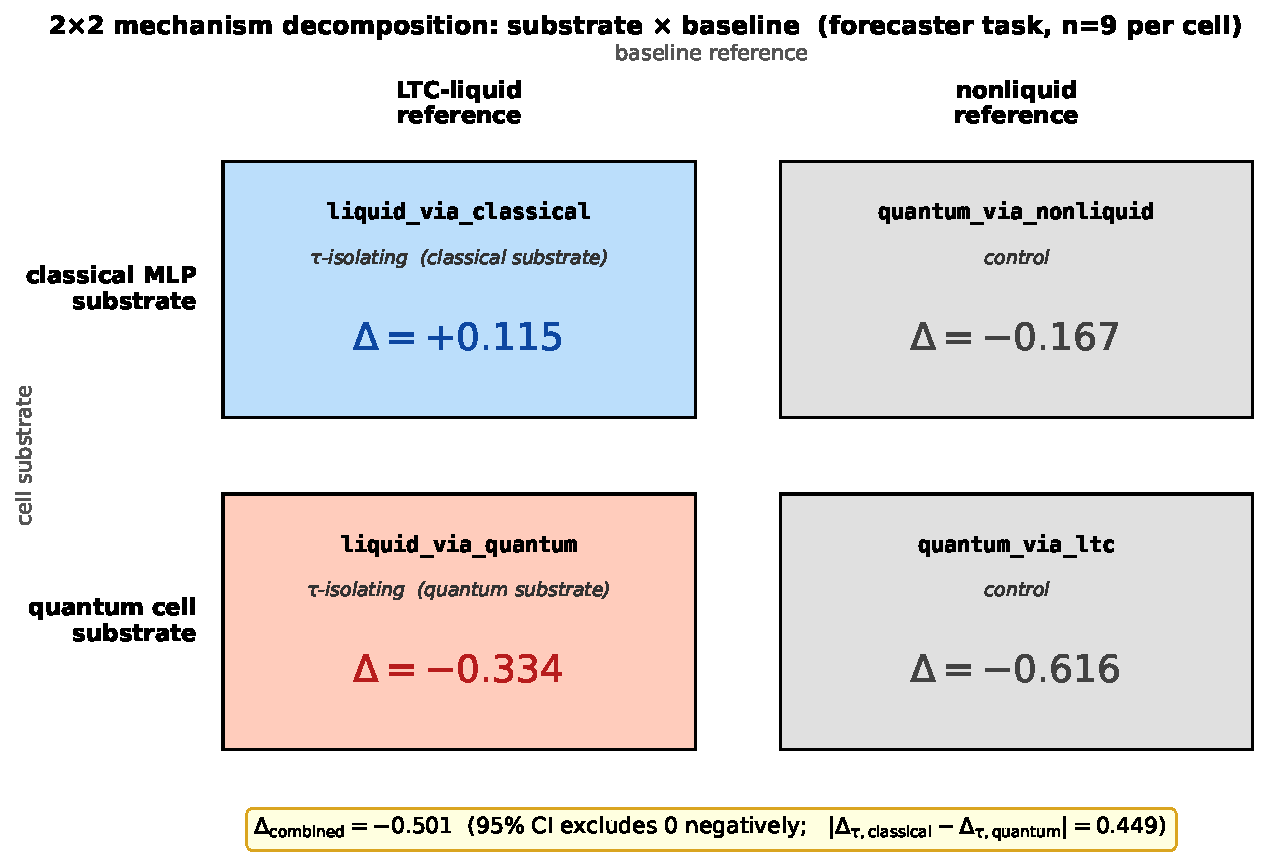
\includegraphics[width=\columnwidth]{figures/fig_2x2_decomposition.pdf}
\caption{The 2$\times$2 mechanism-decomposition design introduced by
amendments A12--A13. Rows index the cell substrate (classical MLP
vs.\ quantum cell); columns index the baseline reference (LTC-liquid
vs.\ nonliquid Neural-ODE). The four per-cell $\Delta_{\mathrm{diff}}$
algebraically partition the headline forecaster
$\Delta_{\mathrm{combined}} = -0.501$ into substrate and reference
contributions plus an interaction term -- the substrate-dependent
$\tau$ signature analyzed in Figure~\ref{fig:tau-substrate}.}
\label{fig:2x2-cartoon}
\end{figure}

\begin{figure}[t]
\centering
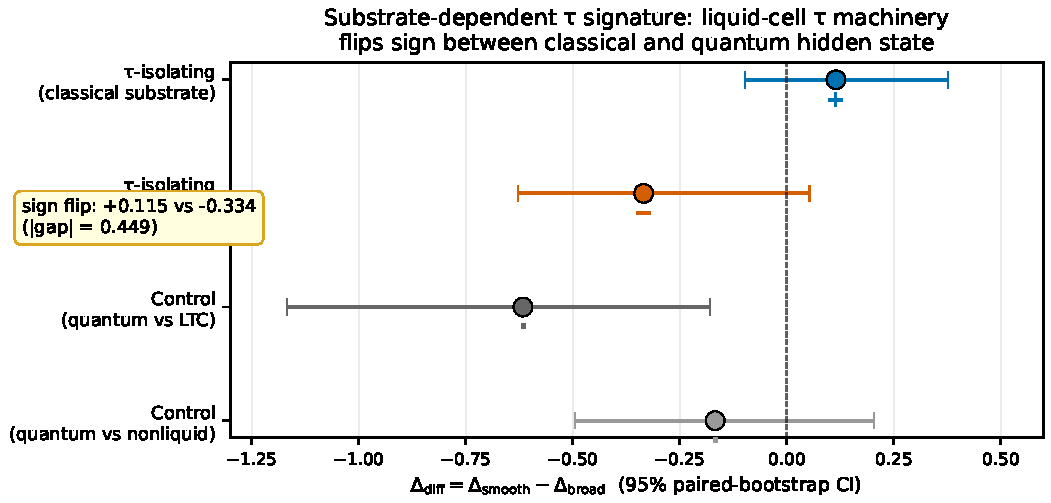
\includegraphics[width=\columnwidth]{figures/fig_tau_substrate.pdf}
\caption{Substrate-dependent $\tau$ signature: the two decomposition
paths that \emph{isolate} the liquid time-constant machinery
(\texttt{liquid\_via\_classical}, \texttt{liquid\_via\_quantum})
disagree in sign, with $|\Delta_{\mathrm{classical}} -
\Delta_{\mathrm{quantum}}| \approx 0.449$. The two control paths
(\texttt{quantum\_via\_ltc}, \texttt{quantum\_via\_nonliquid}), which
do \emph{not} isolate $\tau$, are both negative and broadly consistent
with the combined verdict. This is the paper's strongest mechanistic
evidence that LTC-style time-constant machinery interacts with the
substrate it is mounted on, and the seed for a planned follow-up paper
(Section~\ref{sec:discussion}).}
\label{fig:tau-substrate}
\end{figure}

\begin{figure*}[t]
\centering
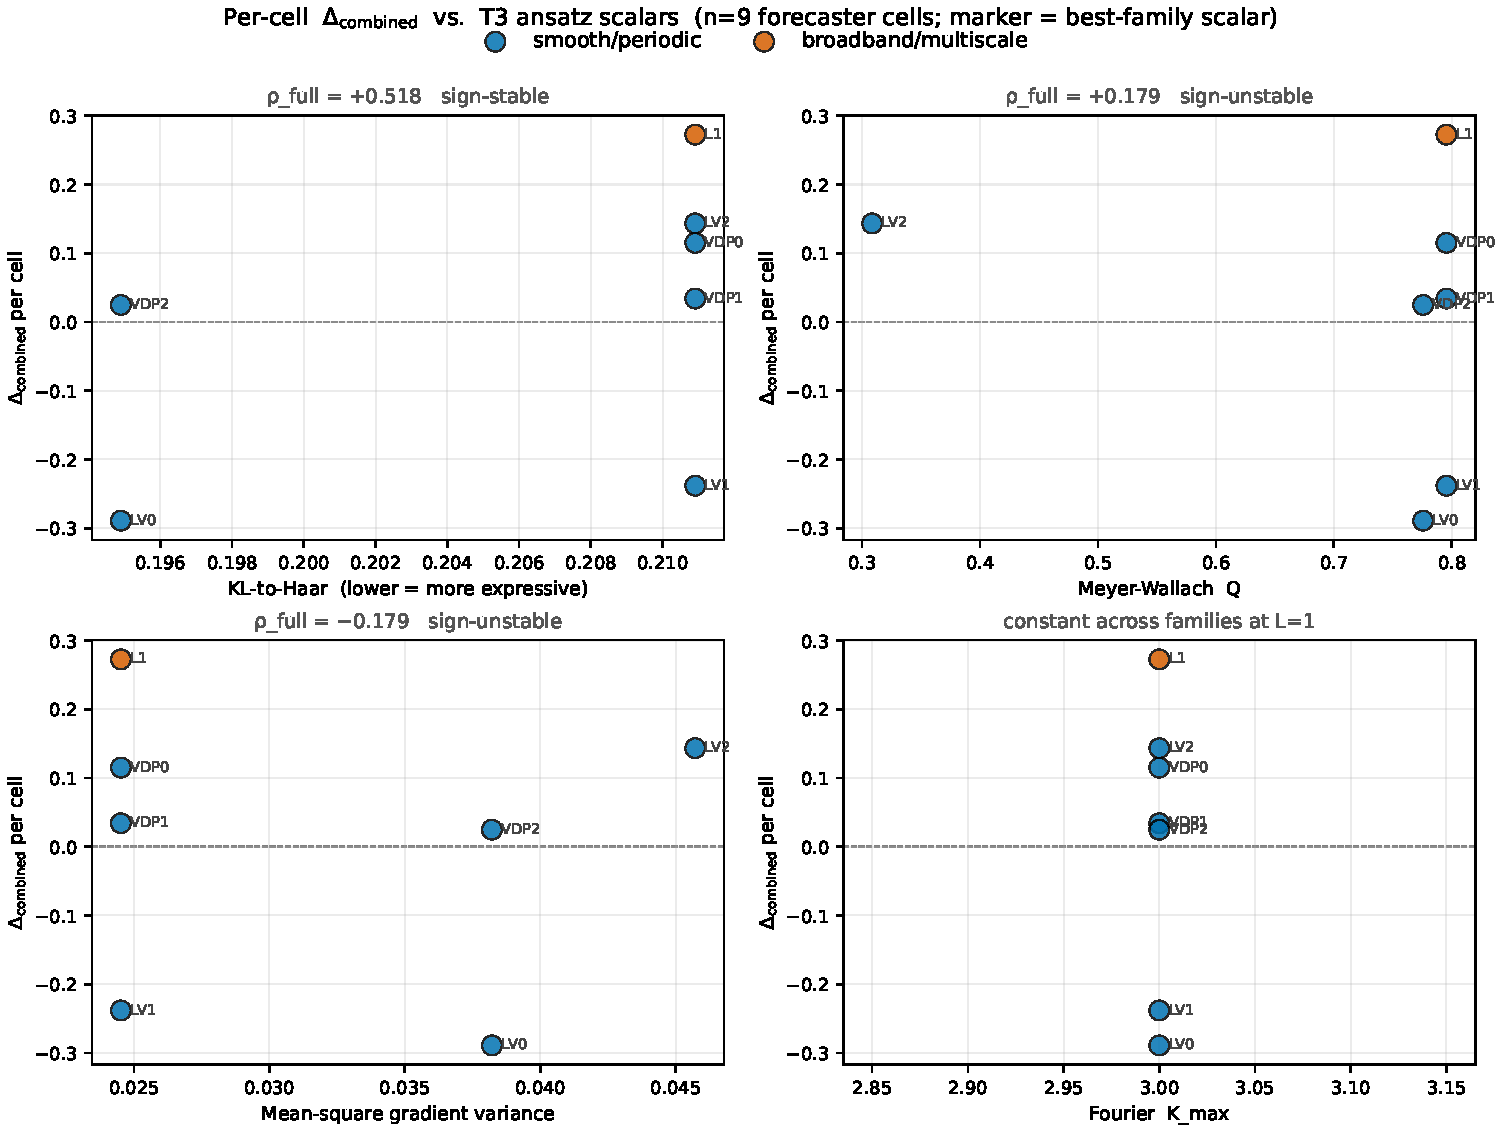
\includegraphics[width=0.95\textwidth]{figures/fig_delta_vs_t3_scatter.pdf}
\caption{Per-cell $\Delta_{\mathrm{combined}}$ scattered against each
of the four T3 ansatz scalars (KL-to-Haar, Meyer--Wallach $Q$,
mean-square gradient variance, Fourier $K_{\max}$) at the cell's
best-quantum family. Color encodes regime (blue =
smooth/periodic; orange = broadband/multiscale); marker labels are
abbreviated (system, seed). The KL-to-Haar panel (top-left) is the
only one with a sign-stable trend ($\rho_{\mathrm{full}} = +0.518$,
all-9 LOO resamples positive); Meyer--Wallach $Q$ and gradient
variance (top-right, bottom-left) carry weak unstable trends; Fourier
$K_{\max}$ (bottom-right) is degenerate at $L=1$. The scatter exposes
the $n=9$ caveat: even the sign-stable trend rests on a 9-point spread.}
\label{fig:delta-vs-t3}
\end{figure*}

\begin{figure*}[t]
\centering
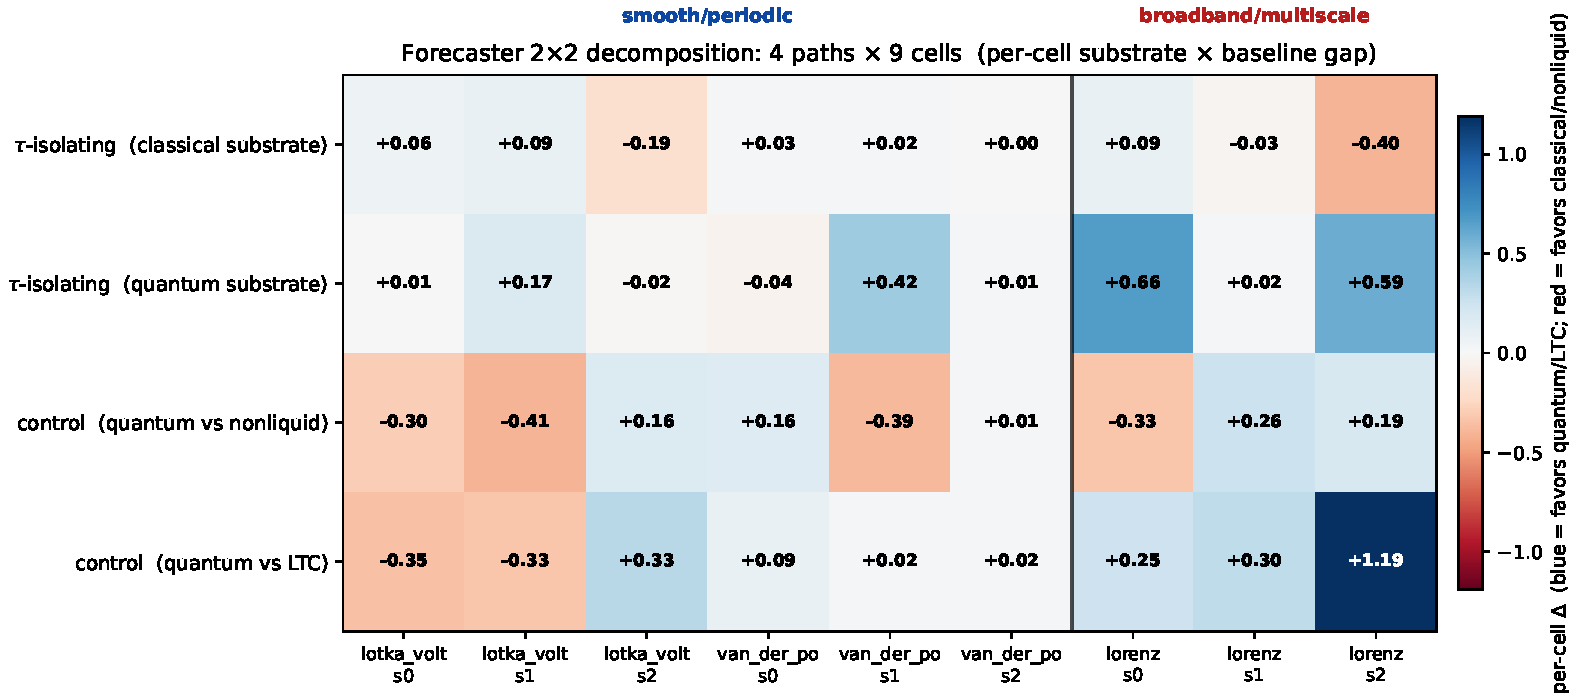
\includegraphics[width=0.95\textwidth]{figures/fig_forecaster_2x2_heatmap.pdf}
\caption{Forecaster 2$\times$2 decomposition, per-cell breakdown.
Rows are the four decomposition paths
(Section~\ref{sec:forecaster-decomp}); columns are the nine
(system, seed) cells, with the regime band labeled at the top.
Blue cells favor the
quantum/LTC side of the contrast; red cells favor the classical/non-liquid
side. The substrate-dependent $\tau$ signature
(Figure~\ref{fig:tau-substrate}) is visible at the per-cell level:
the second row (\texttt{liquid\_via\_quantum}) carries the strong
broadband-positive cells (lorenz s0 = $+0.66$, lorenz s2 = $+0.59$),
while the controls (rows 3-4) split between negative smooth cells
and positive broadband cells, consistent with the $-0.501$ aggregate
verdict and the broadband-leaning sign on the solver task.}
\label{fig:forecaster-heatmap}
\end{figure*}

\subsection{Connecting the mechanism story to the LTC decomposition}
\label{sec:mechanism-ltc}

The mechanism cross-tabulation and the P7.10 LTC decomposition agree on
the locus: \emph{the quantum circuit is the active component} in the
regime-contrast inversion. The liquid-time-constant
cell~\cite{hasani2021liquid,hasani2022closed} is itself a Neural
ODE~\cite{chen2018neural,rubanova2019latent} with a learned $\tau$ on
the hidden state; the 2$\times$2 decomposition (rows = substrate $\tau$
rides on, columns = baseline reference) partitions the headline
$\Delta_{\mathrm{combined}}$ into substrate, reference, and interaction
contributions. The quantum-isolated $\Delta = -0.616$, CI $[-1.167,
-0.178]$ (significantly negative) lies on the quantum-substrate row,
where H3 also shows the within-quantum-roster pattern (data-reuploading,
the most expressive circuit at lowest KL, attains the largest mean
positive per-cell $\Delta$).

Neither finding rescues the pre-registered $H_1$ direction; both
identify the quantum circuit as the mechanism. The follow-up paper
(Section~\ref{sec:discussion}) pursues this directly: P7.7's hardening
techniques (Quantum Natural Gradient, causal training weighting, higher
reuploading depth) are precisely the interventions that would shift
per-cell $\Delta$ via the KL-to-Haar mechanism, if the
expressivity-helps reading is correct.

\begin{figure}[t]
\centering
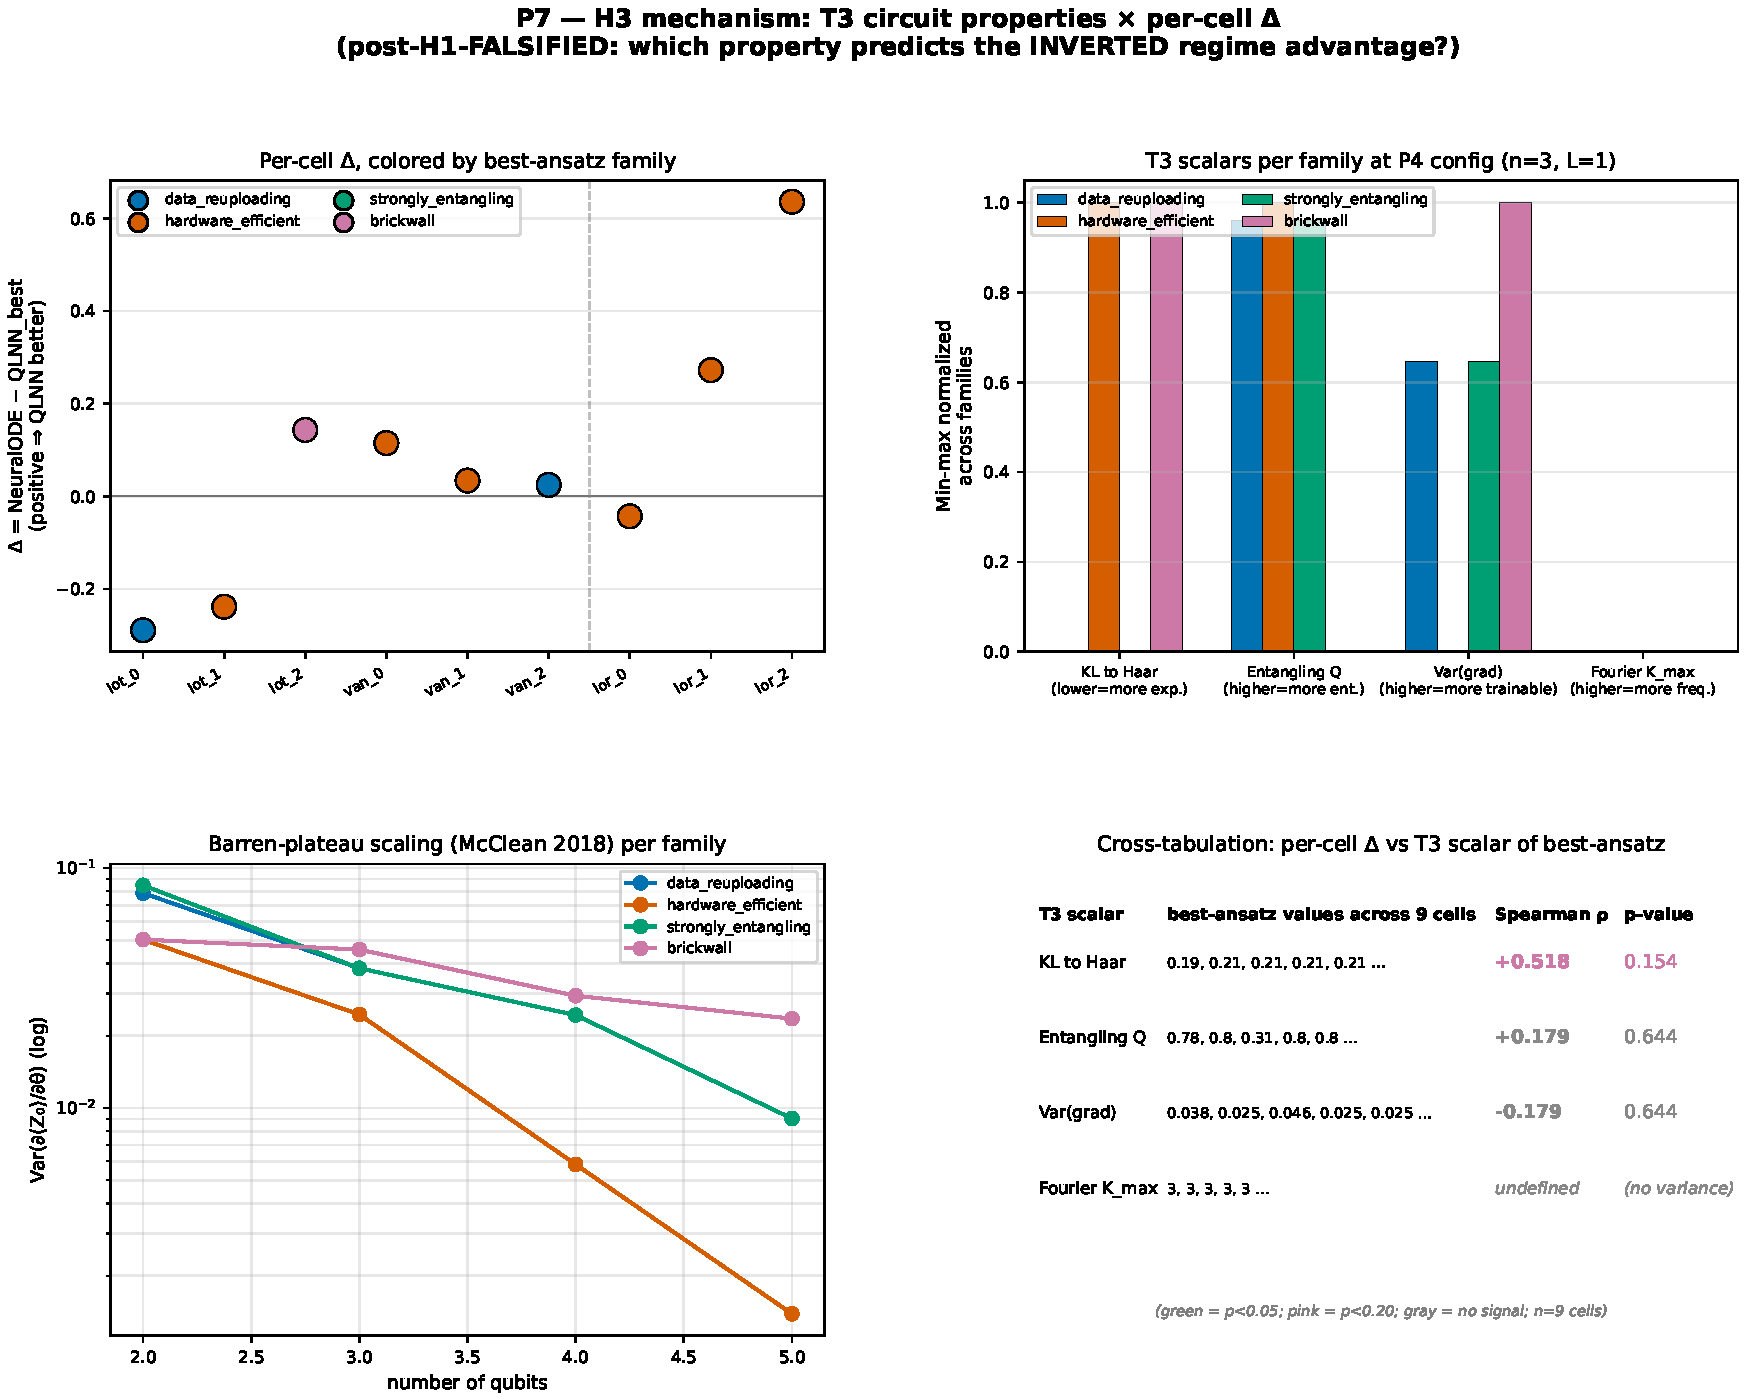
\includegraphics[width=\columnwidth]{figures/fig_p7_mechanism.pdf}
\caption{$H_3$ mechanism cross-tabulation: per-family T3 scalars
(Meyer--Wallach $Q$, KL-to-Haar divergence, gradient variance, Fourier
$K_{\max}$) versus per-cell $\Delta$ on the forecaster task. KL-to-Haar
(lower $=$ more expressive) is the only scalar with a sign-stable
leave-one-out trend ($\rho = +0.518$, all 9 LOO resamples positive).}
\label{fig:mechanism}
\end{figure}
